%!TEX root = ../../report.tex
\chapter{State of the art} % (fold)
\label{cha:state_of_the_art}
This chapter contains a concise overview of some of the major, and more relevant for this thesis, advances in artificial legged locomotion in the past 60 years.
To do so, a brief prelude of the emergence and evolution of natural, limb-based terrestrial motion and more in detail bipedalism is presented.
It is followed by a short introduction of some of the results recorded in history from the union between the engineering field and the study of motion and legged systems. 
From the first, ancient mobile artifacts and prosthesis to the current, most advanced systems in robotics.
And it finishes with an exposition of three of the most pertinent breakthroughs in modern technologies that allowed to reach the current state of the art in modern autonomous walking robots.

%!TEX root = ../../../report.tex
\section{The evolution of bipedalism}
\label{sec:bipedalism}

The current human bipedal locomotion arises from the combination of a wide variety of subsystems working in conjunction to achieve the intended gait generation according to the requirements of the situation.
The biomechanics of the limbs, consisting in bones, muscles and tendons under the control of the nervous system yields the adequate production of the different motion patterns in order to displace the body as energetically efficiently as possible.
This complex behavior is the result of 4 million years of an evolution \cite{bipedalism2} that started in primates and that has entailed both morphological and neurological changes in the human body since the first bipedal hominids to the current structure in Homo sapiens.
There exist several different theories about the reasons that originated and led to the adaption of this posture and bipedal motion.
Although different, most of them assume that most of them assume that the development of this structural and behavioral changes arose from a change in the environment in pre-hominids, for with bipedal behavior suddenly offered some kind of survival value \cite{bipedalism1}.
However, the genus Homo is not the only species that has evolved towards two-legged locomotion
Currently there are a few more species that have reached this method of displacement as a result of a natural selection process in which bipedalism offered the broadest set of advantages of the specie being the main ones listed below. 

\\
\hfill

\begin{itemize}
	\item Erect posture for a wider field of view and reach range.
	\item Free forelimbs, that could evolve towards specialized, non-locomotory applications such as object manipulation, combat, flight, etc.
	\item Faster displacement in certain species, although not generally.
\end{itemize}

Extensive research in the actuation and control structures involved in human bipedalism has been conducted from within the scientific fields of anthropology, biology, medicine, sport science and lately, several areas withing the engineering.
Its goal, as per definition of science, has been to reach a full understanding of what led to this behavior and the knowledge of how it functions, together with the discovery of ways in which it can be mimicked and improved, aiming at a more inexpensive and optimized locomotion.
This last fact has led to the belief that the next stage in the evolution of human locomotion will not come from nature as until nowadays, but from the hand of science and engineering, which has been lately depicted in literature and pop-culture as in \ref{fig:biped_evolution}.

\begin{figure}[h]
	\centering
	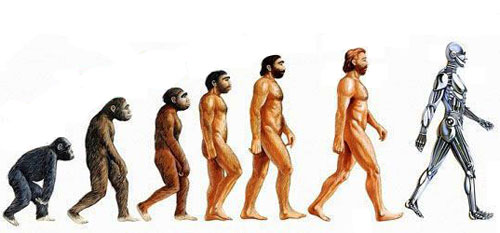
\includegraphics[width=0.8\textwidth]{figures/artificialhumans.jpg}
	\caption{Evolution of bipedalism (artistic depiction from \cite{human_evol_fig})}
	\label{fig:biped_evolution}
\end{figure}

\subsection{Biped motion and engineering} % (fold)
\label{sub:bipedalism_and_engineering}
The discipline of engineering has been historically among the latest of the cited ones to start its contribution to the research and improvement of biped motion in a well defined manner, although its earliest contributions seem to date from ancient Egypt and India \cite{prosthetics_history}.
From the study of human bipedal motion described above, the insights emerged regarding its biomechanical and control functioning together with the need to restore, improve or imitate its capabilities led to the creation of new branches within the discipline of engineering.
The three most relevant ones for the present thesis are listed and introduced below.

\begin{enumerate}
	\item Orthotics
	\item Prosthetics
	\item Artificial legged locomotion 
\end{enumerate}

\paragraph{Orthotics} % (fold)
\label{par:orthotics}
Orthotics is a specialty within the medical field concerned with the design, manufacture and application of orthoses. An orthosis is an externally applied device used to modify the structural and functional characteristics of the neuromuscular and skeletal system, as per definition in \cite{ISO_orthosis}.

Therapeutic models to exoskeletons... 
\todo{Add some more stuff}
% paragraph orthotics (end)

\paragraph{Prosthetics} % (fold)
\label{par:prosthetics}
Prosthetics is the field of medicine that comprises the design and creation of prosthesis, defined as artificial limbs aimed at restoring motor and sensory capabilities in amputee patients.
Since the first lower-limb prosthesis implant recorded in history, documented in the Rigveda \cite{prosthetics_history}, to the current state of the art there has been more than 3000 years of development.
This time has taken prosthetics from single-piece, non-articulated devices with no actuation or sensory feedback to the current near-natural, anthropomorphic structures and control systems adapted to the patient needs and able to closely provide the properties of a biological limb.
As in the orthoses design, the aim of the prosthetics is to mimic as closely as possible the human capabilities with designs such that they adapt to the subject as naturally as possible.
Thus, their development goes parallel to the research and understanding of the human body.
One of the most comprehensive studies in lower-limb prostheses, their design and actuation is the one provided in \cite{grimmer}.
% paragraph prosthetics (end)

\begin{figure}[h]
	\centering
    \begin{subfigure}[b]{0.3\textwidth}
        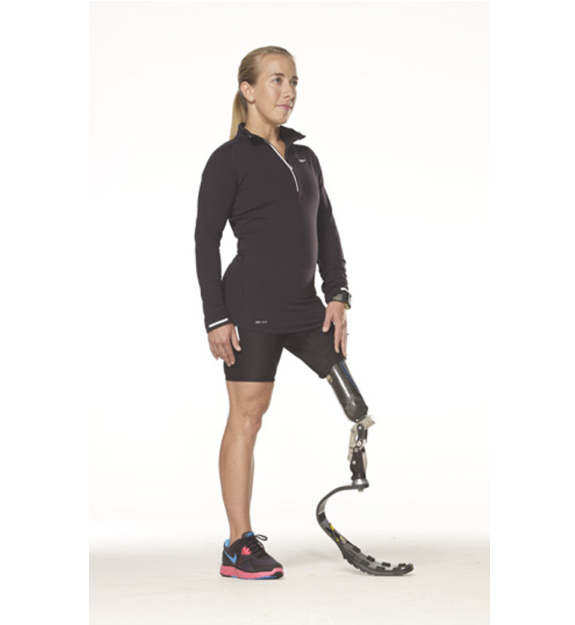
\includegraphics[width=\textwidth]{figures/prosthetic_leg.pdf}
        \caption{Prosthetic leg, Össur Flex-Run}
        \label{fig:prosthetic_leg}
    \end{subfigure}
    \centering
    \begin{subfigure}[b]{0.3\textwidth}
        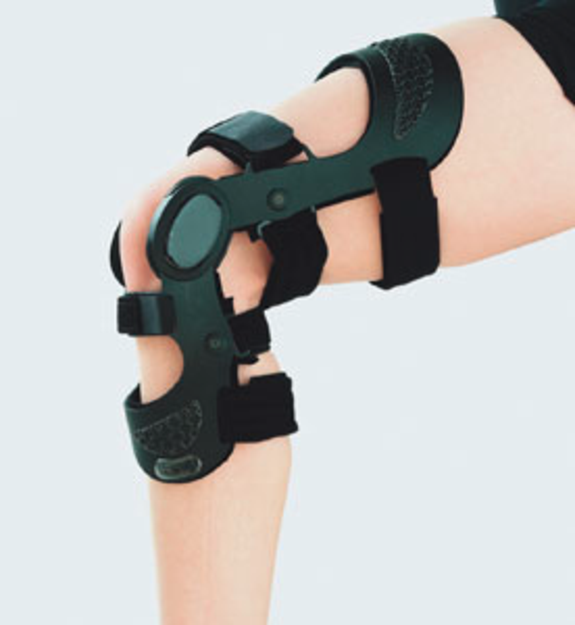
\includegraphics[width=\textwidth]{figures/orthotic_leg.pdf}
        \caption{Knee orthosis, New Hope Co.}
        \label{fig:orthotic_leg}
    \end{subfigure}
    \centering
    \begin{subfigure}[b]{0.3\textwidth}
        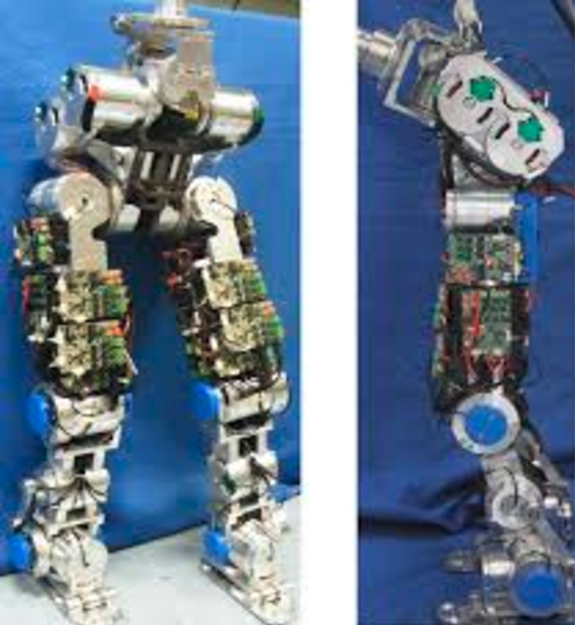
\includegraphics[width=\textwidth]{figures/robotic_leg.pdf}
        \caption{Robotic legs, COMAN robot \cite{coman}}
        \label{fig:robotic_leg}
    \end{subfigure}
\end{figure}

\paragraph{Artificial legged locomotion} % (fold)
\label{par:humanoid_robots}  
The first artificial walking artifacts recorded date from the ancient Greece.
It is in this period when humankind first tries to imitate and replicate the structures found in nature, creating mechanisms to get a deeper knowledge of their functioning and mimic them.
But it is during the Renaissance in Europe when the developments in mechanics and the study of the nature and the human body allows to create the first automata able to walk as a predefined combination of complex mechanical operations.
It is after the Second World War, with the application of electronics and computer technology that the advancement of walking machines is revolutionized \cite{legged_mot_history1}.

The engineering branch of modern robotics has its origins in the second half of the 20th century has a conjunction of the areas of electrical and mechanical engineering and computer science.
However, its interest in achieving resemblance to the locomotion means of both humans and animals  and their capabilities arose in the 1980's.
It first crystallized into the construction of Wabot-1 at WASEDA University or the creation of the Leg Laboratory by Marc Raibert at the Massachusetts Technological Institute.
The purpose of the research in this field was the construction of useful knowledge basis on how human and animal locomotion works that could be used in the creation of legged vehicles, as described in \cite{mit_leg_lab1}.
% paragraph humanoid_robots (end)



% subsection bipedalism_and_engineering (end)


%!TEX root= ../../../report.tex

\section{From the wheel to the leg} % (fold)
\label{sec:from_the_wheel_to_the_leg}
While the wheel is a young human invention meant to facilitate terrestrial motion, legged locomotion has been the result of millions of years of adaption of the species from the aquatic to a terrestrial field.
During this time, even though other forms of motion on the ground emerged, including limbless or rolling, the tetrapod and quadrupedal motion are the ones that have proved the best performances in terrestrial displacements in terms of relative velocity or jump length, for instance.

\subsection{Discovering the wheel (in robotics)} % (fold)
\label{sub:the_wheel_in_robotics}
Despite the facts above, it was the wheel the mean chosen to implement the ability to move around on the first mobile robots such as Walter's tortoises or the John Hopkins University robot Beast \cite{first_mobile_robot}, \cite{second_mobile_robot}.
This could be explained due to the fact that, as an artificial human creation, the modeling and control of the wheel could be fully mastered during its evolution process, easing its implementation in robotic platforms.
Some examples of this are shown in Figure \ref{fig:mobile_robots}, which depicts three current applications of the wheel in robot platforms.

Although the wheel was chosen as the motion mean to face what can be considered one of the most challenging and unpredictable environment a robot can be subject to, the surface of a new planet, it was not the only option. 
The Space General Corporation firstly studied the use of multi-legged autonomous platforms for lunar exploration in the early 1960's \cite{legged_mot_history1}.
However, their use was eventually discarded due to its poor adaptability due to a too low number of DOF.
The "Spirit" robot in \ref{fig:mobile_rover}, within the NASA's Mars Exploration Rover mission, is the example of the current solution to extraplanetary exploration and a good example of the possibilities and limits entailed by wheel-based locomotion.
It was successfully launched on Mars surface in 2004 and it stayed active and operative until 2010.
However, the end of the mission came from the hand of the terrain. 
A very low-cohesion area of soil made the wheels of the device loose traction and eventually get trapped, preventing from recovering the control of the vehicle and bringing about the end of the mission.

Figure \ref{fig:mobile_mir} shows a MIR 100 robot, a state-of-the-art service robot designed for independent transportation and logistics in a dynamic and unpredictable environment..
As a service robot, it must fulfill strict safety standards and guarantee a secure interaction with users and other equipment while accomplishing its tasks.
Thanks to its wheels configuration, it can achieve an agile mobility, fast reaction capacity and a big load capacity.

The EMIEW 2, in \ref{fig:mobile_hitachi}, is an example of midpoint between wheeled and legged locomotion.
Although its motion relies on steering wheels, their placement at the end of two leg-like lower-limbs provides with some of the advantages of bipedal motion, such as active suspension or impact absorption.

\begin{figure}[h]
\label{fig:mobile_robots}
	\centering
    \begin{subfigure}[b]{0.32\textwidth}
        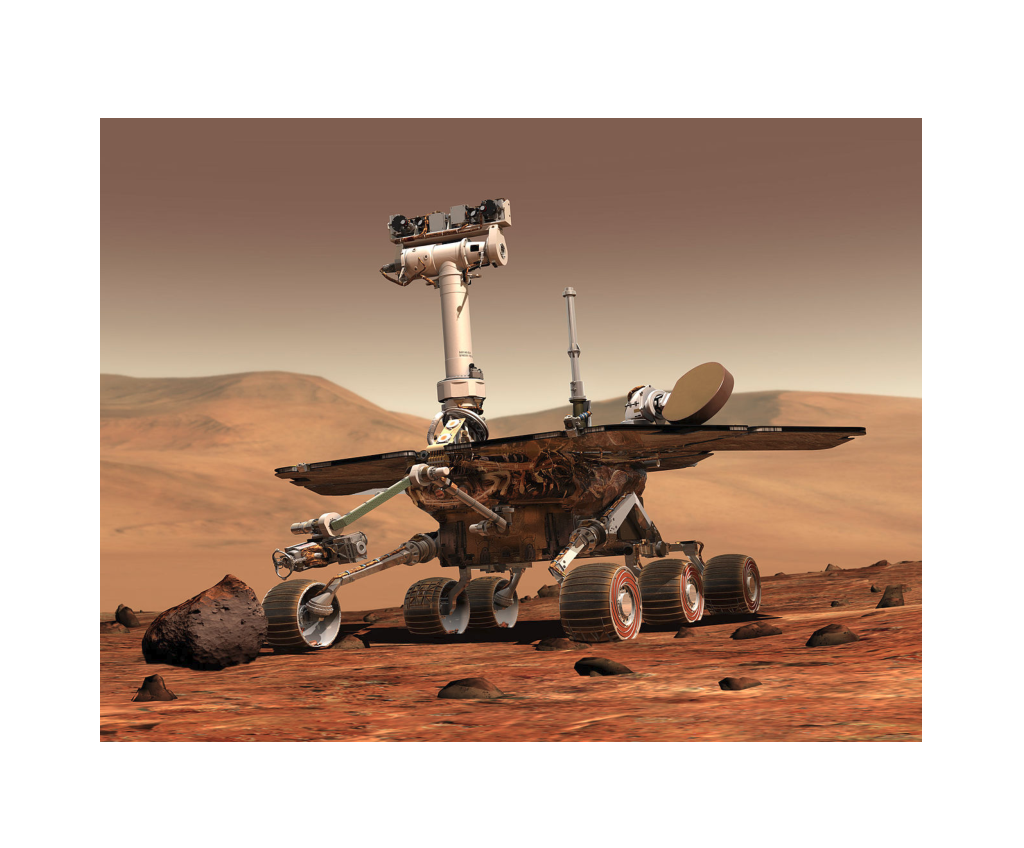
\includegraphics[width=\textwidth]{figures/mobile_rover.pdf}
        \caption{Mars Rover Spirit}
        \label{fig:mobile_rover}
    \end{subfigure}
    \centering
    \begin{subfigure}[b]{0.32\textwidth}
        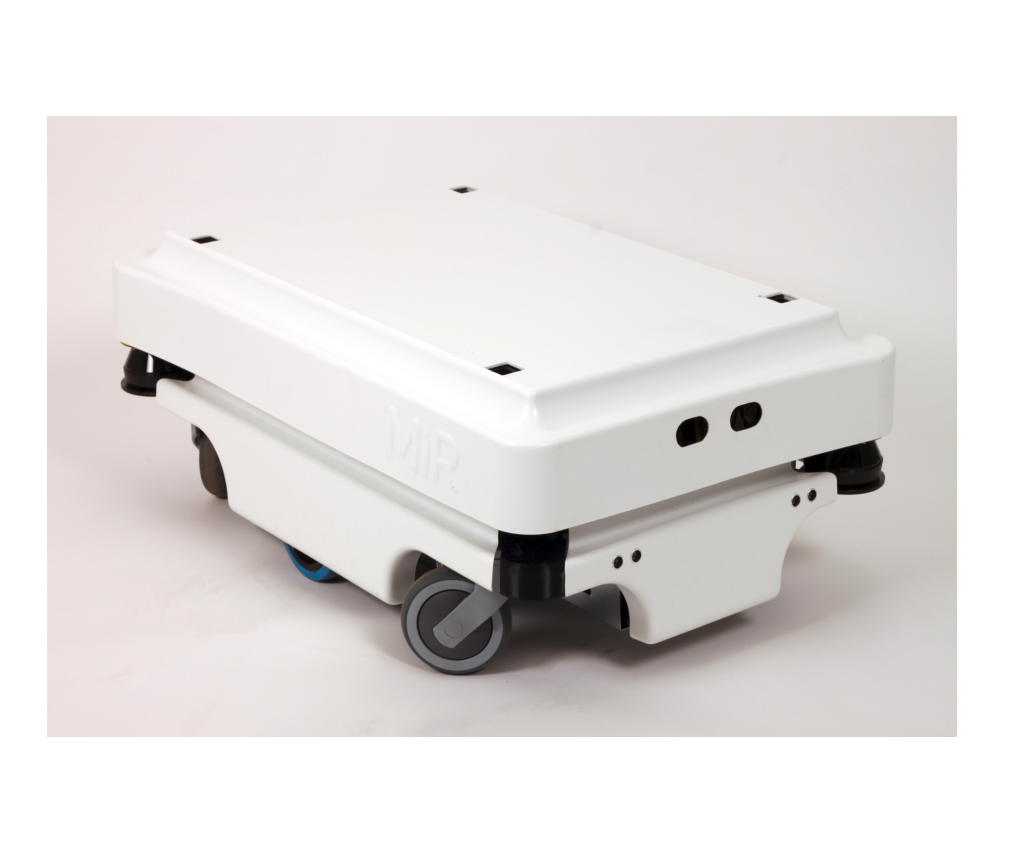
\includegraphics[width=\textwidth]{figures/mobile_mir.pdf}
        \caption{MIR 100 by MIR}
        \label{fig:mobile_mir}
    \end{subfigure}
    \centering
    \begin{subfigure}[b]{0.32\textwidth}
        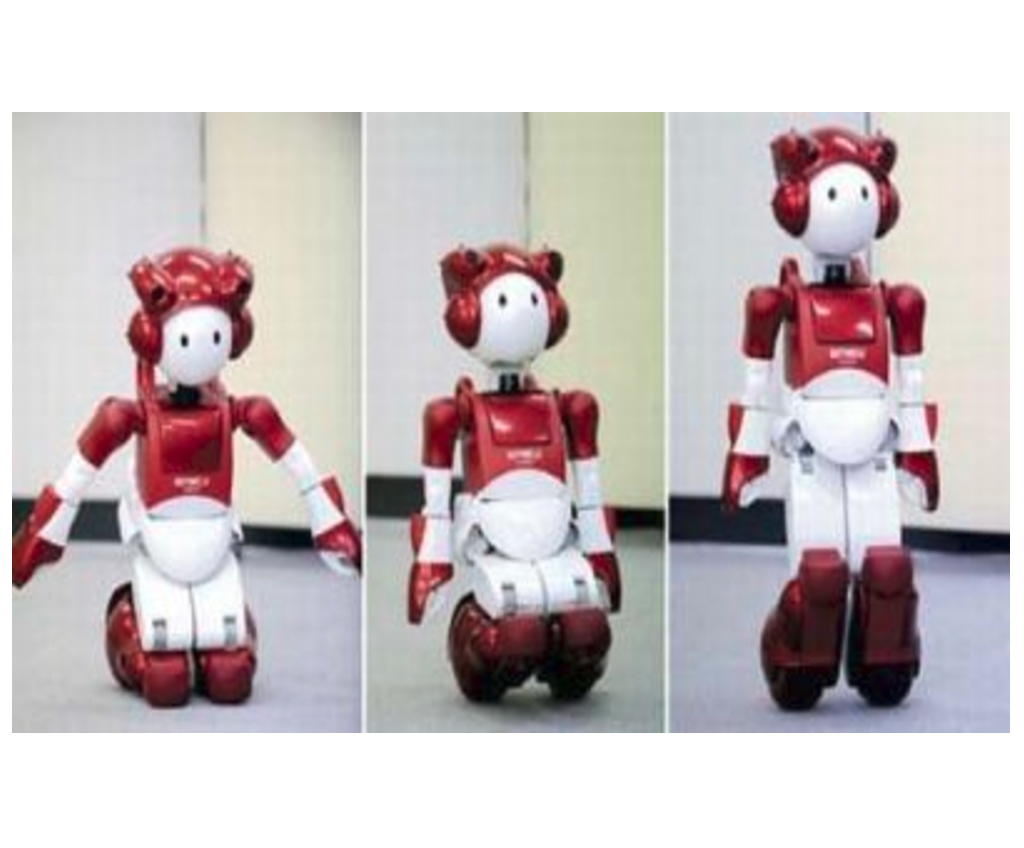
\includegraphics[width=\textwidth]{figures/mobile_hitachi.pdf}
        \caption{EMIEW2, by Hitachi}
        \label{fig:mobile_hitachi}
    \end{subfigure}
\end{figure}

% subsection the_wheel_in_robotics (end)

\subsection{Achieving legged motion} % (fold)
\label{sub:legged_motion_in_robotics}
In spite of the great successes attained in the field of wheeled-robotics, possible thanks to the development in engines and the increasing computing capacity of embedded processors, mobile robots based on wheels have not been able to achieve performances in motion comparable to the ones found in nature.
Specially in uneven terrains, velocity, maneuverability, and efficiency are still problems under study.
Besides, the absence of wheels in nature as a result of darwinian evolution ultimately led to questioning \cite{dawkins} if they are truly the best mean to overcome the challenges that displacements in uneven, unknown surfaces yield for robots.
In words of Richard Dawkins \cite{dawkins} "[the wheel] is dependent for maximum efficiency on a prior invention – the road (or other smooth, hard surface)". 
Figure \ref{fig:biped_robots} contains three of the most advanced stages in legged locomotion nowadays.
They have been chosen because they are meaningful current paradigms of what brought about the revolution to the leg-based locomotion systems in the 80's: the conjunction between mechanics and control as the producers of the expected behavior \cite{mit_leg_lab1}.

The STARLeth robot in \ref{fig:starleth}, built at the Autonomous System Lab at ETH, is an example of robot legged robot inspired by nature. 
It is meant at proving that versatility, speed, robustness and efficiency can be achieved together in a legged moving platform \cite{starleth}.
But it also represents the control problems arisen from this kind of locomotion, by definition unstable and complex (12 actuated joints and 6 unactuated DOF). 

In Figure \ref{fig:kaist} the Raptor robot created at KAIST is shown.
This robot is inspired in a velociraptor structure and has been able to achieve a top stable speed on a treadmill of 46 $km/h$, making it the current fastest biped robot (although the Cheetah robot by Boston Dynamics has the record with a quadruped).
However, it is discussed here because of its simple bioinspired design, which combines prosthetic blades with a dynamic tail for stabilization and only required two motors.
This makes it a good illustration of the importance of biomechanics in the overall system.

Finally the ATLAS robot by Boston Dynamics, in \ref{fig:atlas}, represents the state of the art in bipedal autonomous platforms handling unknown, rough terrain and its interaction with dynamically changing environment.
This task for a high degree of freedom mobile manipulator as a humanoid requires a very robust interactive motion planning and control in order to quickly carry out its assignment while overcoming unpredicted situations fast and reliably enough.
The ATLAS is a good illustration of the relevance of a robust but flexible and adaptive control architecture for this kind of machines.


\begin{figure}[h]
\label{fig:biped_robots}
	\centering
    \begin{subfigure}[b]{0.32\textwidth}
        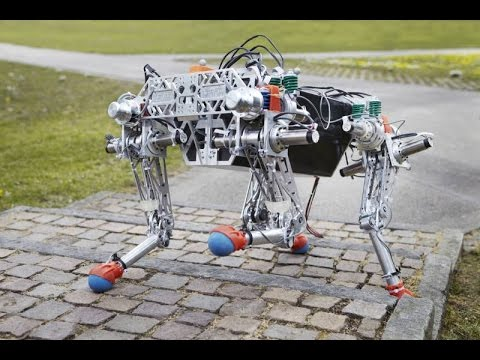
\includegraphics[width=\textwidth]{figures/starleth.jpg}
        \caption{STARLeth}
        \label{fig:starleth}
    \end{subfigure}
    \centering
    \begin{subfigure}[b]{0.32\textwidth}
        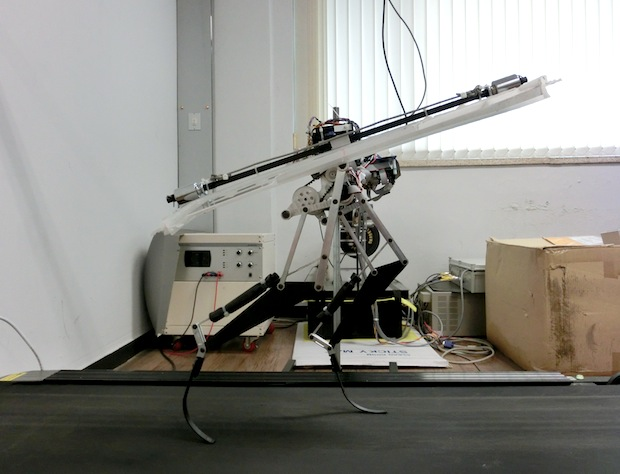
\includegraphics[width=\textwidth]{figures/biped_kaist.jpg}
        \caption{Raptor}
        \label{fig:kaist}
    \end{subfigure}
    \centering
    \begin{subfigure}[b]{0.32\textwidth}
        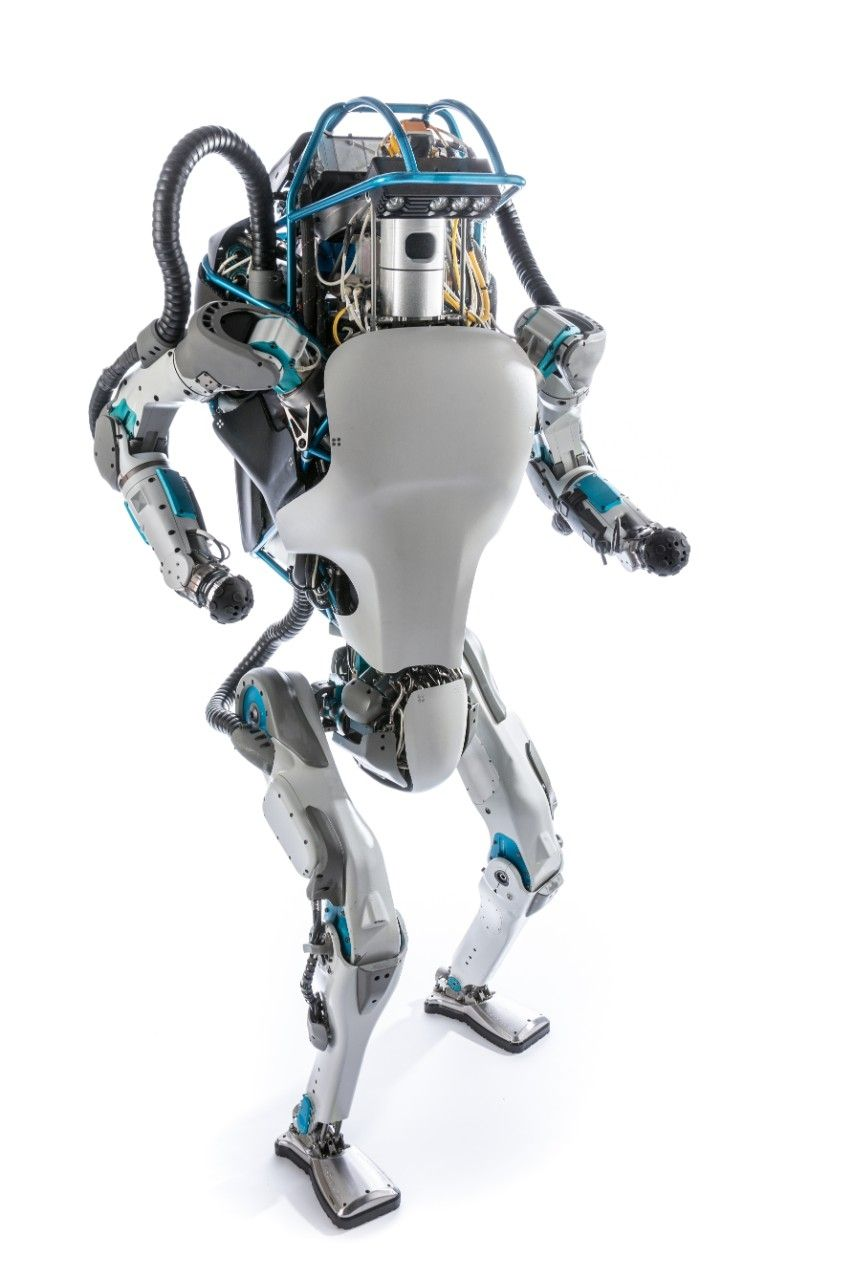
\includegraphics[width=\textwidth]{figures/biped_atlas.jpg}
        \caption{ATLAS}
        \label{fig:atlas}
    \end{subfigure}
\end{figure}


% subsection legged_motion_in_robotics (end)





% section from_the_wheel_to_the_leg (end)
%!TEX root= ../../../report.tex

\section{Biomechanics meets Control} % (fold)
\label{sec:biomechanics_vs_control}
The first attempts to accomplish artificial walking machines in the mid-1950s were based on stiff structures and kinematic control.
There has been more than 50 years of development in several technology fields between them and the current soft, compliant and torque-controlled legged robots.
Among the main advances that gave rise to the evolution of the autonomous walking robots, three considered essential and of great relevance for this thesis are listened in \ref{list:leg_advances} and further discussed here.
Thanks to them, nowadays the research in legged robotics goes hand in hand with the study of biological locomotion systems in the attempt to imitate existing features present in nature.

\begin{itemize}
\label{list:leg_advances}
	\item The realization of the importance that a dynamic and active control has on the walking behavior, as opposed to rigid, kinematics-based motion.
	\item The conception of the embodied AI. The influence of the body in the process of thinking.
	\item The improvements in sensors/actuators performance, material science, embedded computing power and power sources.
\end{itemize}

\subsection{The relevance of body dynamics} % (fold)
\label{sub:dynamics_control}
Stiff position control for kinematic trajectory planning has lately demonstrated impressive capabilities for instance during the last DARPA learning locomotion challenge.
However, the limitations of this kind of control such as the need of a very detailed knowledge  about both the robot state vector and the environment have been also exposed.
Thus, it seems clear that the solution for robust and adaptive motion platforms has to go through the development of dynamics-based control models.
The first big steps in dynamic legged locomotion control took place in the 90's in the Leg Laboratory, at the MIT Artificial Intelligence Laboratory carried out by Marc Raibert and his team.
Their findings about the importance of active balance for stability and the possibility of creating simple and generalizable control algorithms for complex dynamic legged systems \cite{mit_leg_lab1} pushed the development of walking robots to a new stage.
Besides, they were among the pioneers in the realization of the influence of the mechanical design together with the control in the generation of complex behaviors in locomotion.
A paradigmatic example of the importance of the biomechanics and the body dynamics in the control of machines intended for locomotion is the well-known passive walker developed by McGeer \cite{passive_walking} and shown in \ref{fig:passive_walker}. 
The achievement of a human-like, efficient walking behavior without any kind control structure gave birth to the concept of morphological computation.

% subsection dynamics_control (end)
\begin{figure}[h]
	\centering
	\begin{subfigure}[b]{0.45\textwidth}
        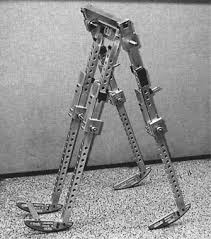
\includegraphics[width=\textwidth]{figures/passive_walker.jpg}
        \caption{McGeer passive walker}
        \label{fig:passive_walker}
    \end{subfigure}
    \begin{subfigure}[b]{0.45\textwidth}
        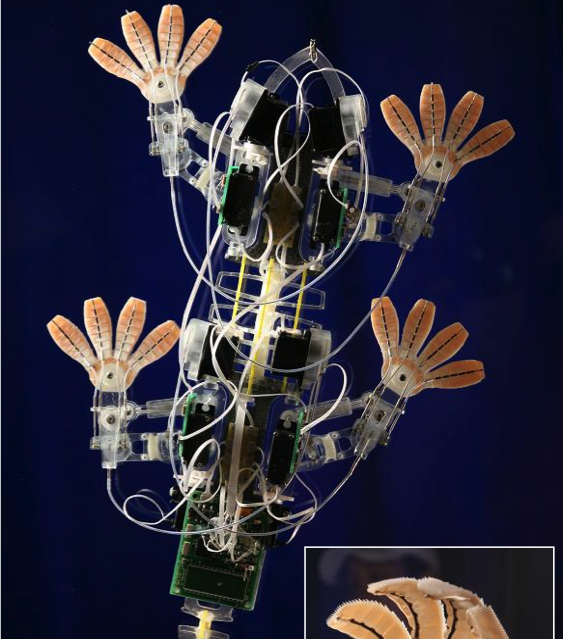
\includegraphics[width=\textwidth]{figures/Stickybot.jpg}
        \caption{Stickybot robot, Standford University}
        \label{fig:stickybot}
    \end{subfigure}
\caption{Examples of bio inspired mechanics in locomotion}
\label{fig:figure1}
\end{figure}

\subsection{Embodied AI and locomotion} % (fold)
\label{sub:the_embodiment_}
The embodiment concept came up in the Artificial Intelligence field in the 1980's as a mean to explore the influence of the body and its characteristics in the process of thinking. 
Its aim could be expressed as the search for the answer to the question, in the very convenient words of Rolf Pfeifer and Fumiya Iida, "How does walking relate to thinking?".
As introduced in \cite{pfeifer}, the original goal of AI the understanding of natural forms of intelligence that have more to do with the interaction with the real world rather than the only development of computer algorithms.

The advent of this new approach in AI caused by itself an enormous boost in the field of locomotion in robotics since it made researchers start working with mobile robots.
"The general initial conviction that locomotion and orientation were the underlying driving forces in the development of cognition, in the evolution of the brain, led to the general use of the already available wheeled robots" \cite{pfeifer}.
In the seek of an answer to the famous question "Why don’t plants have brains?", by D. Wolpert, the belief that the reason could be their incapacity for displacement led to an increasing use of mobile robots as a research tool.

Besides, the embodied AI brought about the turn to nature for inspiration in biological systems under the belief that the results of Darwinian evolution and the principle of ecological balance had created systems of greater complexity and optimality worth studying and mimicking.
With all this, it came the understanding that complex behavior could arise from the synergistic combination of simple algorithms and the physical characteristics of the body.
Since then, mechanical compliance in the actuation, soft materials and bio inspired controllers such as CPGs for instance have been widely studied and implemented in walking machines. 
An example of this concept is the Stickybot, created in the Biomimetics and Dexterous Manipulation Lab at Standford University and shown in Figure \ref{fig:stickybot}.
% subsection the_embodiment_ (end)

\subsection{Main advances in hardware} % (fold)
\label{sub:the_advances_in_hardware}



% (1) nonavailability of energy-efficient and high-performance actuators with high torque to weight ratio and high torque to volume ratio; 
% (2) reliable and economical sensors; (3) lightweight but mechanically strong
% material for construction of the structure and mechanism; (4) fast, high computing
% power, and economical dedicated computer system that must be suitable for any
% type of hostile situation of nature; and (5) lightweight and onboard power source for
% long duration energy autonomy.

%First WAP robots bipedalism_history pag 28

% subsection the_advances_in_hardware (end)


% section biomechanics_vs_control (end)
%!TEX root= ../../../report.tex

\section{The next generation of bipeds} % (fold)
\label{sec:the_next_generation_of_bipeds}
It appears clear now that the evolution of bipedal locomotion has in the last decades suffered a wide-reaching change in its conditions with the entrance on the stage of robotics science and its research in walking machines.
It still stands difficult, however, to foresee the paths that the advancements in artificial bipedalism will take without the risk of getting lost in speculations.
Notwithstanding, the latest breakthroughs yield reasons to believe that the next generation of walking machines will resemble more and more the physiological designs developed by nature, although only to the extent that the state-of-the-art mechantronics allows.
This last fact entails that a complete imitation of living biological structures is yet out of the reach of engineering, thus making its goal not to just copy, but to understand the underlying principles that drive biology and transfer them to the new synthetic creations with the existing technology.



However, the latest advances in some of the youngest areas of the engineering seem to be close to bring about a change in the so far unaltered rules of the game.
The progresses in AI and in the design of genetic algorithms have arisen the possibility of not only striving for mimicking nature, but also replicating its fundamental processes, artificially accelerating and modifying them.
In the next decades, nature could stop being the only motor of evolution and from there, the possibilities are boundless.

% section the_next_generation_of_bipeds (end)
%%!TEX root = ../../report.tex
\chapter{State of the art} % (fold)
\label{cha:state_of_the_art}
%!TEX root = ../../../report.tex
\section{The evolution of bipedalism}
\label{sec:bipedalism}

The current human bipedal locomotion arises from the combination of a wide variety of subsystems working in conjunction to achieve the intended gait generation according to the requirements of the situation.
The biomechanics of the limbs, consisting in bones, muscles and tendons under the control of the nervous system yields the adequate production of the different motion patterns in order to displace the body as energetically efficiently as possible.
This complex behavior is the result of 4 million years of an evolution \cite{bipedalism2} that started in primates and that has entailed both morphological and neurological changes in the human body since the first bipedal hominids to the current structure in Homo sapiens.
There exist several different theories about the reasons that originated and led to the adaption of this posture and bipedal motion.
Although different, most of them assume that most of them assume that the development of this structural and behavioral changes arose from a change in the environment in pre-hominids, for with bipedal behavior suddenly offered some kind of survival value \cite{bipedalism1}.
However, the genus Homo is not the only species that has evolved towards two-legged locomotion
Currently there are a few more species that have reached this method of displacement as a result of a natural selection process in which bipedalism offered the broadest set of advantages of the specie being the main ones listed below. 

\\
\hfill

\begin{itemize}
	\item Erect posture for a wider field of view and reach range.
	\item Free forelimbs, that could evolve towards specialized, non-locomotory applications such as object manipulation, combat, flight, etc.
	\item Faster displacement in certain species, although not generally.
\end{itemize}

Extensive research in the actuation and control structures involved in human bipedalism has been conducted from within the scientific fields of anthropology, biology, medicine, sport science and lately, several areas withing the engineering.
Its goal, as per definition of science, has been to reach a full understanding of what led to this behavior and the knowledge of how it functions, together with the discovery of ways in which it can be mimicked and improved, aiming at a more inexpensive and optimized locomotion.
This last fact has led to the belief that the next stage in the evolution of human locomotion will not come from nature as until nowadays, but from the hand of science and engineering, which has been lately depicted in literature and pop-culture as in \ref{fig:biped_evolution}.

\begin{figure}[h]
	\centering
	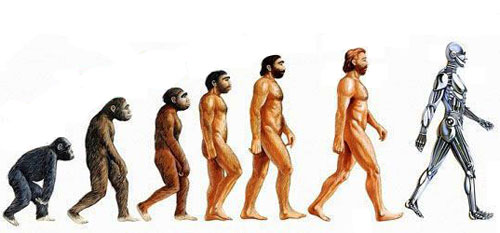
\includegraphics[width=0.8\textwidth]{figures/artificialhumans.jpg}
	\caption{Evolution of bipedalism (artistic depiction from \cite{human_evol_fig})}
	\label{fig:biped_evolution}
\end{figure}

\subsection{Biped motion and engineering} % (fold)
\label{sub:bipedalism_and_engineering}
The discipline of engineering has been historically among the latest of the cited ones to start its contribution to the research and improvement of biped motion in a well defined manner, although its earliest contributions seem to date from ancient Egypt and India \cite{prosthetics_history}.
From the study of human bipedal motion described above, the insights emerged regarding its biomechanical and control functioning together with the need to restore, improve or imitate its capabilities led to the creation of new branches within the discipline of engineering.
The three most relevant ones for the present thesis are listed and introduced below.

\begin{enumerate}
	\item Orthotics
	\item Prosthetics
	\item Artificial legged locomotion 
\end{enumerate}

\paragraph{Orthotics} % (fold)
\label{par:orthotics}
Orthotics is a specialty within the medical field concerned with the design, manufacture and application of orthoses. An orthosis is an externally applied device used to modify the structural and functional characteristics of the neuromuscular and skeletal system, as per definition in \cite{ISO_orthosis}.

Therapeutic models to exoskeletons... 
\todo{Add some more stuff}
% paragraph orthotics (end)

\paragraph{Prosthetics} % (fold)
\label{par:prosthetics}
Prosthetics is the field of medicine that comprises the design and creation of prosthesis, defined as artificial limbs aimed at restoring motor and sensory capabilities in amputee patients.
Since the first lower-limb prosthesis implant recorded in history, documented in the Rigveda \cite{prosthetics_history}, to the current state of the art there has been more than 3000 years of development.
This time has taken prosthetics from single-piece, non-articulated devices with no actuation or sensory feedback to the current near-natural, anthropomorphic structures and control systems adapted to the patient needs and able to closely provide the properties of a biological limb.
As in the orthoses design, the aim of the prosthetics is to mimic as closely as possible the human capabilities with designs such that they adapt to the subject as naturally as possible.
Thus, their development goes parallel to the research and understanding of the human body.
One of the most comprehensive studies in lower-limb prostheses, their design and actuation is the one provided in \cite{grimmer}.
% paragraph prosthetics (end)

\begin{figure}[h]
	\centering
    \begin{subfigure}[b]{0.3\textwidth}
        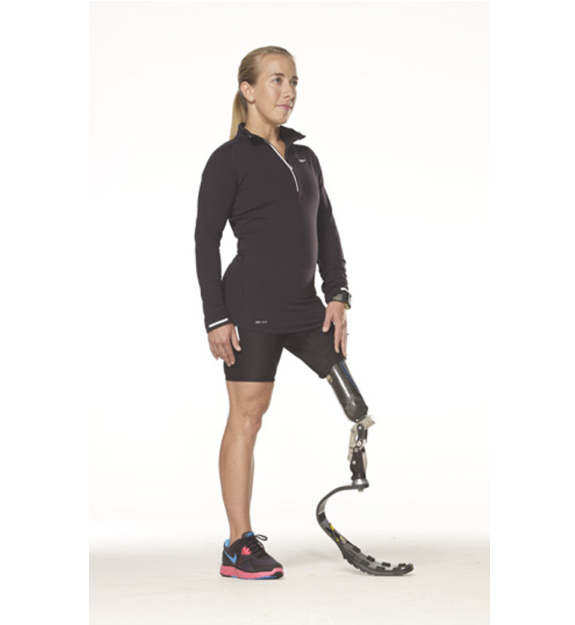
\includegraphics[width=\textwidth]{figures/prosthetic_leg.pdf}
        \caption{Prosthetic leg, Össur Flex-Run}
        \label{fig:prosthetic_leg}
    \end{subfigure}
    \centering
    \begin{subfigure}[b]{0.3\textwidth}
        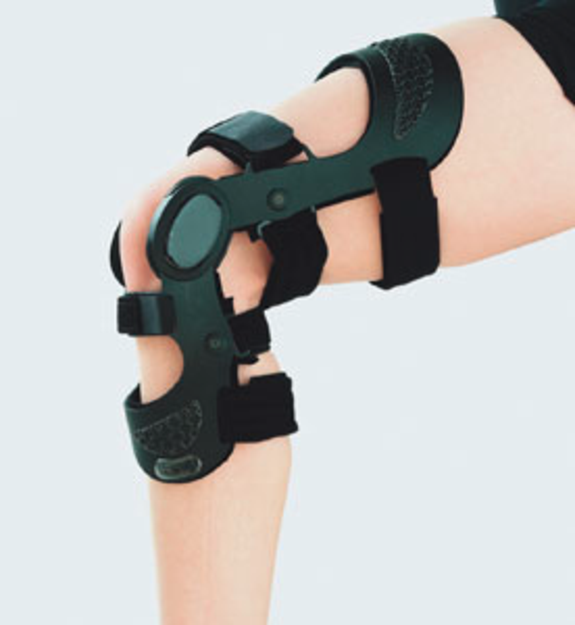
\includegraphics[width=\textwidth]{figures/orthotic_leg.pdf}
        \caption{Knee orthosis, New Hope Co.}
        \label{fig:orthotic_leg}
    \end{subfigure}
    \centering
    \begin{subfigure}[b]{0.3\textwidth}
        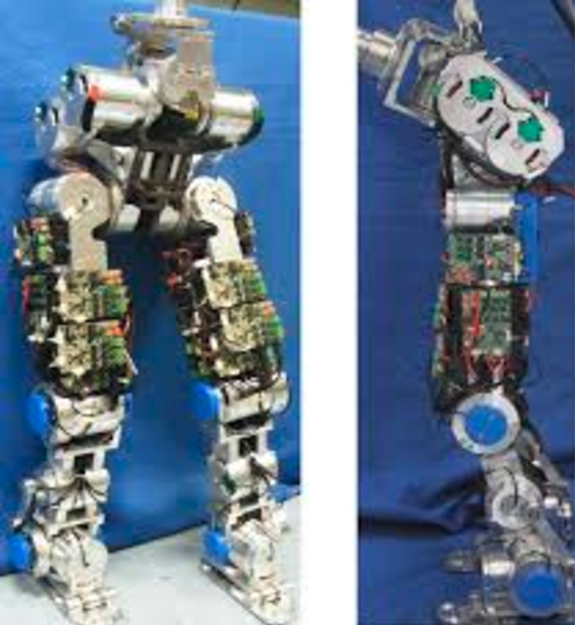
\includegraphics[width=\textwidth]{figures/robotic_leg.pdf}
        \caption{Robotic legs, COMAN robot \cite{coman}}
        \label{fig:robotic_leg}
    \end{subfigure}
\end{figure}

\paragraph{Artificial legged locomotion} % (fold)
\label{par:humanoid_robots}  
The first artificial walking artifacts recorded date from the ancient Greece.
It is in this period when humankind first tries to imitate and replicate the structures found in nature, creating mechanisms to get a deeper knowledge of their functioning and mimic them.
But it is during the Renaissance in Europe when the developments in mechanics and the study of the nature and the human body allows to create the first automata able to walk as a predefined combination of complex mechanical operations.
It is after the Second World War, with the application of electronics and computer technology that the advancement of walking machines is revolutionized \cite{legged_mot_history1}.

The engineering branch of modern robotics has its origins in the second half of the 20th century has a conjunction of the areas of electrical and mechanical engineering and computer science.
However, its interest in achieving resemblance to the locomotion means of both humans and animals  and their capabilities arose in the 1980's.
It first crystallized into the construction of Wabot-1 at WASEDA University or the creation of the Leg Laboratory by Marc Raibert at the Massachusetts Technological Institute.
The purpose of the research in this field was the construction of useful knowledge basis on how human and animal locomotion works that could be used in the creation of legged vehicles, as described in \cite{mit_leg_lab1}.
% paragraph humanoid_robots (end)



% subsection bipedalism_and_engineering (end)


%%!TEX root = ../../report.tex
\chapter{State of the art} % (fold)
\label{cha:state_of_the_art}
%!TEX root = ../../../report.tex
\section{The evolution of bipedalism}
\label{sec:bipedalism}

The current human bipedal locomotion arises from the combination of a wide variety of subsystems working in conjunction to achieve the intended gait generation according to the requirements of the situation.
The biomechanics of the limbs, consisting in bones, muscles and tendons under the control of the nervous system yields the adequate production of the different motion patterns in order to displace the body as energetically efficiently as possible.
This complex behavior is the result of 4 million years of an evolution \cite{bipedalism2} that started in primates and that has entailed both morphological and neurological changes in the human body since the first bipedal hominids to the current structure in Homo sapiens.
There exist several different theories about the reasons that originated and led to the adaption of this posture and bipedal motion.
Although different, most of them assume that most of them assume that the development of this structural and behavioral changes arose from a change in the environment in pre-hominids, for with bipedal behavior suddenly offered some kind of survival value \cite{bipedalism1}.
However, the genus Homo is not the only species that has evolved towards two-legged locomotion
Currently there are a few more species that have reached this method of displacement as a result of a natural selection process in which bipedalism offered the broadest set of advantages of the specie being the main ones listed below. 

\\
\hfill

\begin{itemize}
	\item Erect posture for a wider field of view and reach range.
	\item Free forelimbs, that could evolve towards specialized, non-locomotory applications such as object manipulation, combat, flight, etc.
	\item Faster displacement in certain species, although not generally.
\end{itemize}

Extensive research in the actuation and control structures involved in human bipedalism has been conducted from within the scientific fields of anthropology, biology, medicine, sport science and lately, several areas withing the engineering.
Its goal, as per definition of science, has been to reach a full understanding of what led to this behavior and the knowledge of how it functions, together with the discovery of ways in which it can be mimicked and improved, aiming at a more inexpensive and optimized locomotion.
This last fact has led to the belief that the next stage in the evolution of human locomotion will not come from nature as until nowadays, but from the hand of science and engineering, which has been lately depicted in literature and pop-culture as in \ref{fig:biped_evolution}.

\begin{figure}[h]
	\centering
	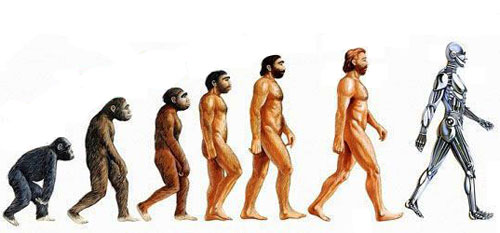
\includegraphics[width=0.8\textwidth]{figures/artificialhumans.jpg}
	\caption{Evolution of bipedalism (artistic depiction from \cite{human_evol_fig})}
	\label{fig:biped_evolution}
\end{figure}

\subsection{Biped motion and engineering} % (fold)
\label{sub:bipedalism_and_engineering}
The discipline of engineering has been historically among the latest of the cited ones to start its contribution to the research and improvement of biped motion in a well defined manner, although its earliest contributions seem to date from ancient Egypt and India \cite{prosthetics_history}.
From the study of human bipedal motion described above, the insights emerged regarding its biomechanical and control functioning together with the need to restore, improve or imitate its capabilities led to the creation of new branches within the discipline of engineering.
The three most relevant ones for the present thesis are listed and introduced below.

\begin{enumerate}
	\item Orthotics
	\item Prosthetics
	\item Artificial legged locomotion 
\end{enumerate}

\paragraph{Orthotics} % (fold)
\label{par:orthotics}
Orthotics is a specialty within the medical field concerned with the design, manufacture and application of orthoses. An orthosis is an externally applied device used to modify the structural and functional characteristics of the neuromuscular and skeletal system, as per definition in \cite{ISO_orthosis}.

Therapeutic models to exoskeletons... 
\todo{Add some more stuff}
% paragraph orthotics (end)

\paragraph{Prosthetics} % (fold)
\label{par:prosthetics}
Prosthetics is the field of medicine that comprises the design and creation of prosthesis, defined as artificial limbs aimed at restoring motor and sensory capabilities in amputee patients.
Since the first lower-limb prosthesis implant recorded in history, documented in the Rigveda \cite{prosthetics_history}, to the current state of the art there has been more than 3000 years of development.
This time has taken prosthetics from single-piece, non-articulated devices with no actuation or sensory feedback to the current near-natural, anthropomorphic structures and control systems adapted to the patient needs and able to closely provide the properties of a biological limb.
As in the orthoses design, the aim of the prosthetics is to mimic as closely as possible the human capabilities with designs such that they adapt to the subject as naturally as possible.
Thus, their development goes parallel to the research and understanding of the human body.
One of the most comprehensive studies in lower-limb prostheses, their design and actuation is the one provided in \cite{grimmer}.
% paragraph prosthetics (end)

\begin{figure}[h]
	\centering
    \begin{subfigure}[b]{0.3\textwidth}
        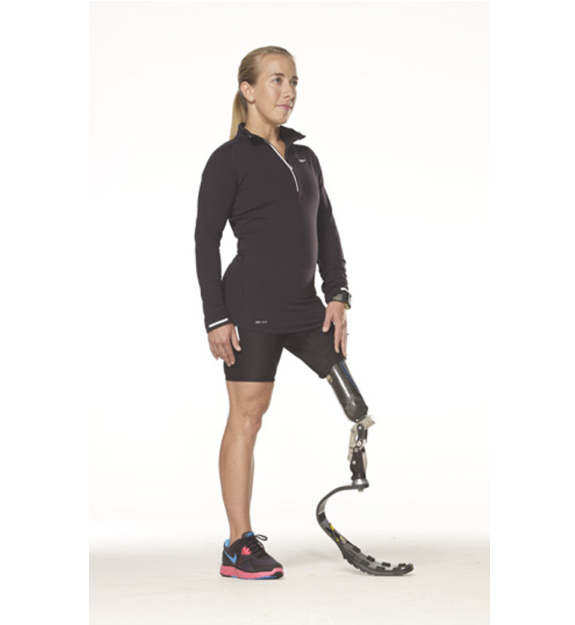
\includegraphics[width=\textwidth]{figures/prosthetic_leg.pdf}
        \caption{Prosthetic leg, Össur Flex-Run}
        \label{fig:prosthetic_leg}
    \end{subfigure}
    \centering
    \begin{subfigure}[b]{0.3\textwidth}
        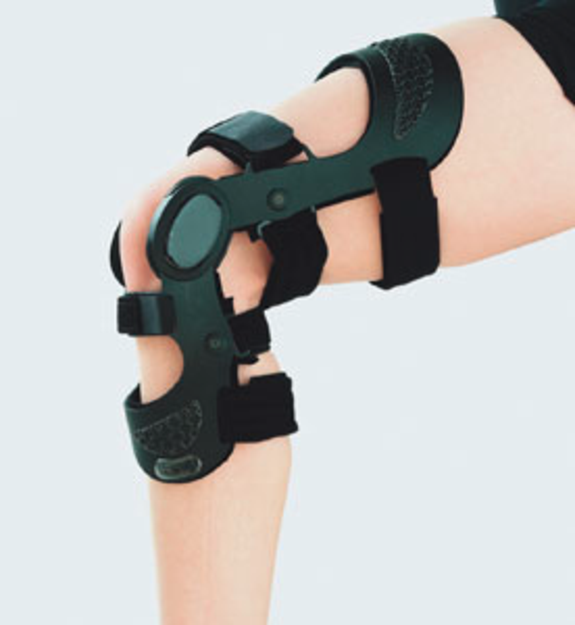
\includegraphics[width=\textwidth]{figures/orthotic_leg.pdf}
        \caption{Knee orthosis, New Hope Co.}
        \label{fig:orthotic_leg}
    \end{subfigure}
    \centering
    \begin{subfigure}[b]{0.3\textwidth}
        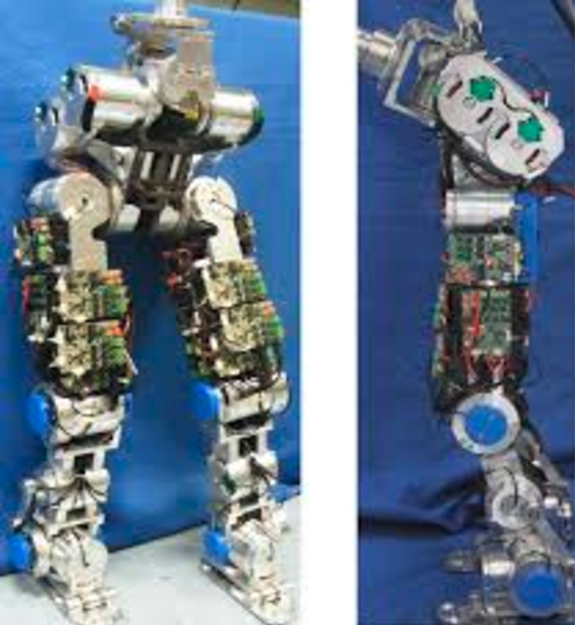
\includegraphics[width=\textwidth]{figures/robotic_leg.pdf}
        \caption{Robotic legs, COMAN robot \cite{coman}}
        \label{fig:robotic_leg}
    \end{subfigure}
\end{figure}

\paragraph{Artificial legged locomotion} % (fold)
\label{par:humanoid_robots}  
The first artificial walking artifacts recorded date from the ancient Greece.
It is in this period when humankind first tries to imitate and replicate the structures found in nature, creating mechanisms to get a deeper knowledge of their functioning and mimic them.
But it is during the Renaissance in Europe when the developments in mechanics and the study of the nature and the human body allows to create the first automata able to walk as a predefined combination of complex mechanical operations.
It is after the Second World War, with the application of electronics and computer technology that the advancement of walking machines is revolutionized \cite{legged_mot_history1}.

The engineering branch of modern robotics has its origins in the second half of the 20th century has a conjunction of the areas of electrical and mechanical engineering and computer science.
However, its interest in achieving resemblance to the locomotion means of both humans and animals  and their capabilities arose in the 1980's.
It first crystallized into the construction of Wabot-1 at WASEDA University or the creation of the Leg Laboratory by Marc Raibert at the Massachusetts Technological Institute.
The purpose of the research in this field was the construction of useful knowledge basis on how human and animal locomotion works that could be used in the creation of legged vehicles, as described in \cite{mit_leg_lab1}.
% paragraph humanoid_robots (end)



% subsection bipedalism_and_engineering (end)


%%!TEX root = ../../report.tex
\chapter{State of the art} % (fold)
\label{cha:state_of_the_art}
\input{chapters/cha_state_of_the_art/Sections/sec_bipedalism_intro}
%\input{chapters/cha_state_of_the_art/cha_state_of_the_art}
%\input{chapters/cha_state_of_the_art/Sections/sec_theoretical_background}
%\section{Theoretical background}



%But it has been in the last 30 years of the past century when the robotics field has started to focus on accomplishing bipedal locomotion, being the first model the WAM-1, built at Waseda University in 1967 \cite{}.
% Since this robot, the evolution of the platforms targeted at mimicking human locomotion has rapidly achieved great successes, which can be exemplified in robots as ASIMO, MABEL or BioBiped \cite{mabel}, \cite{biobiped}, %\cite{}.  
% However, even though the generation of stable walking gaits for biped platforms seems to have reached a next stage with the latest Atlas robot, the variances in kinematics, kinetics and control required for running and for the transition between the walking and running gaits still set out unsolved challenges.
% Besides, differences in energy consumption and balance control or trajectory generation still remain noticeable when comparing the performance of humanoid robots and humans \cite{h7}.

% In order to contribute to the study of stable walking and running gaits generation in bipedal robots, and aiming at providing a new tool to gain new insights on the transition between these gaits, this project offers a new robotic platform for continuing the research in these areas at the University of Southern Denmark.
% The current bipedal robot being utilized at the AI department at the Mærsk Mc-Kinney Møller Institute to benchmark neural controllers for locomotion is the DACbot walking robot, a next generation of RunBot \cite{runbot1} \cite{runbot2}.
% The limitations of this model when trying to approach human-like gait include among others the lack of actuated ankles or compliance in other joints besides the ankles. 
% Furthermore, its fixed structure and the way it was manufactured make modifications for different experiments or even repairs a hard task.
% A new bipedal platform offering a structure easy to modify and repair, low-cost, fully actuated and whose compliant components can be reconfigured, could be a valuable instrument for future studies.
% The RuBi robot, introduced here, wants to be presented as a mean to overcome the above mentioned restrictions and provide these new features. 
% Besides, the possibilities arisen from having two different study platforms in the department include being able to test neural controllers in different robots to observe their adaption, for instance.



%\section{Current research}
% chapter state_of_the_art (end)
%%!TEX root = ../../../report.tex

\section{Theoretical background}
\label{sec:theoretical_background}

%\section{Theoretical background}



%But it has been in the last 30 years of the past century when the robotics field has started to focus on accomplishing bipedal locomotion, being the first model the WAM-1, built at Waseda University in 1967 \cite{}.
% Since this robot, the evolution of the platforms targeted at mimicking human locomotion has rapidly achieved great successes, which can be exemplified in robots as ASIMO, MABEL or BioBiped \cite{mabel}, \cite{biobiped}, %\cite{}.  
% However, even though the generation of stable walking gaits for biped platforms seems to have reached a next stage with the latest Atlas robot, the variances in kinematics, kinetics and control required for running and for the transition between the walking and running gaits still set out unsolved challenges.
% Besides, differences in energy consumption and balance control or trajectory generation still remain noticeable when comparing the performance of humanoid robots and humans \cite{h7}.

% In order to contribute to the study of stable walking and running gaits generation in bipedal robots, and aiming at providing a new tool to gain new insights on the transition between these gaits, this project offers a new robotic platform for continuing the research in these areas at the University of Southern Denmark.
% The current bipedal robot being utilized at the AI department at the Mærsk Mc-Kinney Møller Institute to benchmark neural controllers for locomotion is the DACbot walking robot, a next generation of RunBot \cite{runbot1} \cite{runbot2}.
% The limitations of this model when trying to approach human-like gait include among others the lack of actuated ankles or compliance in other joints besides the ankles. 
% Furthermore, its fixed structure and the way it was manufactured make modifications for different experiments or even repairs a hard task.
% A new bipedal platform offering a structure easy to modify and repair, low-cost, fully actuated and whose compliant components can be reconfigured, could be a valuable instrument for future studies.
% The RuBi robot, introduced here, wants to be presented as a mean to overcome the above mentioned restrictions and provide these new features. 
% Besides, the possibilities arisen from having two different study platforms in the department include being able to test neural controllers in different robots to observe their adaption, for instance.



%\section{Current research}
% chapter state_of_the_art (end)
%%!TEX root = ../../../report.tex

\section{Theoretical background}
\label{sec:theoretical_background}

%\section{Theoretical background}



%But it has been in the last 30 years of the past century when the robotics field has started to focus on accomplishing bipedal locomotion, being the first model the WAM-1, built at Waseda University in 1967 \cite{}.
% Since this robot, the evolution of the platforms targeted at mimicking human locomotion has rapidly achieved great successes, which can be exemplified in robots as ASIMO, MABEL or BioBiped \cite{mabel}, \cite{biobiped}, %\cite{}.  
% However, even though the generation of stable walking gaits for biped platforms seems to have reached a next stage with the latest Atlas robot, the variances in kinematics, kinetics and control required for running and for the transition between the walking and running gaits still set out unsolved challenges.
% Besides, differences in energy consumption and balance control or trajectory generation still remain noticeable when comparing the performance of humanoid robots and humans \cite{h7}.

% In order to contribute to the study of stable walking and running gaits generation in bipedal robots, and aiming at providing a new tool to gain new insights on the transition between these gaits, this project offers a new robotic platform for continuing the research in these areas at the University of Southern Denmark.
% The current bipedal robot being utilized at the AI department at the Mærsk Mc-Kinney Møller Institute to benchmark neural controllers for locomotion is the DACbot walking robot, a next generation of RunBot \cite{runbot1} \cite{runbot2}.
% The limitations of this model when trying to approach human-like gait include among others the lack of actuated ankles or compliance in other joints besides the ankles. 
% Furthermore, its fixed structure and the way it was manufactured make modifications for different experiments or even repairs a hard task.
% A new bipedal platform offering a structure easy to modify and repair, low-cost, fully actuated and whose compliant components can be reconfigured, could be a valuable instrument for future studies.
% The RuBi robot, introduced here, wants to be presented as a mean to overcome the above mentioned restrictions and provide these new features. 
% Besides, the possibilities arisen from having two different study platforms in the department include being able to test neural controllers in different robots to observe their adaption, for instance.



%\section{Current research}
% chapter state_of_the_art (end)
%%!TEX root = ../../../report.tex

\section{Theoretical background}
\label{sec:theoretical_background}

%\section{Theoretical background}



%But it has been in the last 30 years of the past century when the robotics field has started to focus on accomplishing bipedal locomotion, being the first model the WAM-1, built at Waseda University in 1967 \cite{}.
% Since this robot, the evolution of the platforms targeted at mimicking human locomotion has rapidly achieved great successes, which can be exemplified in robots as ASIMO, MABEL or BioBiped \cite{mabel}, \cite{biobiped}, %\cite{}.  
% However, even though the generation of stable walking gaits for biped platforms seems to have reached a next stage with the latest Atlas robot, the variances in kinematics, kinetics and control required for running and for the transition between the walking and running gaits still set out unsolved challenges.
% Besides, differences in energy consumption and balance control or trajectory generation still remain noticeable when comparing the performance of humanoid robots and humans \cite{h7}.

% In order to contribute to the study of stable walking and running gaits generation in bipedal robots, and aiming at providing a new tool to gain new insights on the transition between these gaits, this project offers a new robotic platform for continuing the research in these areas at the University of Southern Denmark.
% The current bipedal robot being utilized at the AI department at the Mærsk Mc-Kinney Møller Institute to benchmark neural controllers for locomotion is the DACbot walking robot, a next generation of RunBot \cite{runbot1} \cite{runbot2}.
% The limitations of this model when trying to approach human-like gait include among others the lack of actuated ankles or compliance in other joints besides the ankles. 
% Furthermore, its fixed structure and the way it was manufactured make modifications for different experiments or even repairs a hard task.
% A new bipedal platform offering a structure easy to modify and repair, low-cost, fully actuated and whose compliant components can be reconfigured, could be a valuable instrument for future studies.
% The RuBi robot, introduced here, wants to be presented as a mean to overcome the above mentioned restrictions and provide these new features. 
% Besides, the possibilities arisen from having two different study platforms in the department include being able to test neural controllers in different robots to observe their adaption, for instance.



%\section{Current research}
% chapter state_of_the_art (end)